\documentclass[]{article}
\usepackage{lmodern}
\usepackage{amssymb,amsmath}
\usepackage{ifxetex,ifluatex}
\usepackage{fixltx2e} % provides \textsubscript
\ifnum 0\ifxetex 1\fi\ifluatex 1\fi=0 % if pdftex
  \usepackage[T1]{fontenc}
  \usepackage[utf8]{inputenc}
\else % if luatex or xelatex
  \ifxetex
    \usepackage{mathspec}
  \else
    \usepackage{fontspec}
  \fi
  \defaultfontfeatures{Ligatures=TeX,Scale=MatchLowercase}
\fi
% use upquote if available, for straight quotes in verbatim environments
\IfFileExists{upquote.sty}{\usepackage{upquote}}{}
% use microtype if available
\IfFileExists{microtype.sty}{%
\usepackage{microtype}
\UseMicrotypeSet[protrusion]{basicmath} % disable protrusion for tt fonts
}{}
\usepackage[margin=1in]{geometry}
\usepackage{hyperref}
\hypersetup{unicode=true,
            pdftitle={Rmarkdown: Word and pdf documents},
            pdfauthor={Sebastien Renaut},
            pdfborder={0 0 0},
            breaklinks=true}
\urlstyle{same}  % don't use monospace font for urls
\usepackage{graphicx,grffile}
\makeatletter
\def\maxwidth{\ifdim\Gin@nat@width>\linewidth\linewidth\else\Gin@nat@width\fi}
\def\maxheight{\ifdim\Gin@nat@height>\textheight\textheight\else\Gin@nat@height\fi}
\makeatother
% Scale images if necessary, so that they will not overflow the page
% margins by default, and it is still possible to overwrite the defaults
% using explicit options in \includegraphics[width, height, ...]{}
\setkeys{Gin}{width=\maxwidth,height=\maxheight,keepaspectratio}
\IfFileExists{parskip.sty}{%
\usepackage{parskip}
}{% else
\setlength{\parindent}{0pt}
\setlength{\parskip}{6pt plus 2pt minus 1pt}
}
\setlength{\emergencystretch}{3em}  % prevent overfull lines
\providecommand{\tightlist}{%
  \setlength{\itemsep}{0pt}\setlength{\parskip}{0pt}}
\setcounter{secnumdepth}{0}
% Redefines (sub)paragraphs to behave more like sections
\ifx\paragraph\undefined\else
\let\oldparagraph\paragraph
\renewcommand{\paragraph}[1]{\oldparagraph{#1}\mbox{}}
\fi
\ifx\subparagraph\undefined\else
\let\oldsubparagraph\subparagraph
\renewcommand{\subparagraph}[1]{\oldsubparagraph{#1}\mbox{}}
\fi

%%% Use protect on footnotes to avoid problems with footnotes in titles
\let\rmarkdownfootnote\footnote%
\def\footnote{\protect\rmarkdownfootnote}

%%% Change title format to be more compact
\usepackage{titling}

% Create subtitle command for use in maketitle
\newcommand{\subtitle}[1]{
  \posttitle{
    \begin{center}\large#1\end{center}
    }
}

\setlength{\droptitle}{-2em}

  \title{Rmarkdown: Word and pdf documents}
    \pretitle{\vspace{\droptitle}\centering\huge}
  \posttitle{\par}
    \author{Sebastien Renaut}
    \preauthor{\centering\large\emph}
  \postauthor{\par}
      \predate{\centering\large\emph}
  \postdate{\par}
    \date{February 06, 2019}


\begin{document}
\maketitle

\section{Microsoft Word}\label{microsoft-word}

\begin{itemize}
\item
  You can specify it when you create a new \texttt{rmarkdown} document.
\item
  You can also specify it later in the YAML header.
\end{itemize}

\texttt{-\/-\/-}\\
\texttt{title:\ "rmarkdown\_pdf\_docx"}\\
\texttt{author:\ "Sebastien\ Renaut"}\\
\texttt{date:\ \textquotesingle{}2018-09-06\textquotesingle{}}\\
\texttt{output:\ word\_document}\\
\texttt{-\/-\/-}

\begin{itemize}
\item
  Then, it's just a matter of kniting the document!
\item
  Little documentation, few options \& configurations are possible.
  (This is not the course of events that should be promoted, as it moves
  away from an open source environment).
\end{itemize}

\section{Portable Document Format
(.pdf)}\label{portable-document-format-.pdf}

\begin{itemize}
\item
  You need a extra step to go from LaTeX (\emph{.tex}) format to a
  \emph{.pdf}. This is handled by the \texttt{pdflatex} function in R.
\item
  \href{https://www.latex-project.org}{LaTeX software} is a high-quality
  typesetting system.
\item
  It is the \emph{de facto} standard for the communication and
  publication of scientific documents.
\item
  LaTeX is available as free software.
\end{itemize}

\begin{figure}
\centering
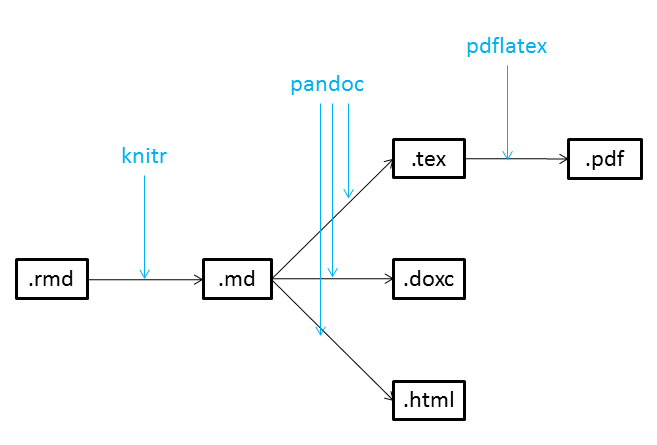
\includegraphics[width=5.20833in]{../figures/pandoc1.png}
\caption{}
\end{figure}

\begin{itemize}
\item
  \href{https://www.latex-project.org/get/}{Latex software} is available
  here.
\item
  If interested, follow this discussion:
  \href{https://ubuntuforums.org/showthread.php?t=395863}{\emph{Why
  LaTeX is such a bloated system?}}
\item
  So\ldots{}\href{https://yihui.name/tinytex/r/}{\emph{TinyTeX}} is a
  custom LaTeX distribution based on TeX Live that is small in size
  (\textasciitilde{}150MB) but functions well in most cases, especially
  for \texttt{R} users .
\item
  \texttt{tinytex} R package is a wrapper function that installs
  \emph{TinyTeX}.
\end{itemize}

\section{Exercice 1 (15min.)}\label{exercice-1-15min.}

\begin{itemize}
\tightlist
\item
  Install the \texttt{tinytex} R package from the console.
\end{itemize}

\begin{quote}
install.packages(``tinytex'')\\
library(tinytex)\\
It takes a few minutes to download and compile tinytex
(\textasciitilde{}150MB)\\
install\_tinytex()
\end{quote}

\begin{itemize}
\tightlist
\item
  Compile your document as \emph{.pdf}:
\end{itemize}

\begin{quote}
---\\
title: ``rmarkdown\_pdf\_docx''\\
author: ``Sebastien Renaut''\\
date: `2018-09-06'\\
output: pdf\_document\\
---
\end{quote}

\section{More complex header}\label{more-complex-header}

\begin{quote}
---\\
output\\
pdf\_document:\\
keep\_tex: true\\
fig\_caption: true\\
latex\_engine: pdflatex\\
title: ``\textbf{This is my first Rmarkdown manuscript}''\\
date: February 06, 2019\\
geometry: margin=1in\\
fontfamily: mathpazo\\
fontsize: 11pt\\
spacing: double\\
csl: ../reference\_material/peerj.csl\\
bibliography: ../reference\_material/reference.bib\\
---
\end{quote}

\begin{itemize}
\item
  Note the indentation in the \textbf{.Rmd} document.
\item
  Note the bibliography file and csl file for formatting references.
\end{itemize}

\section{\texorpdfstring{Exercice 2: R packages \texttt{rticles}
(10min.)}{Exercice 2: R packages rticles (10min.)}}\label{exercice-2-r-packages-rticles-10min.}

\begin{itemize}
\item
  This is a nice package to format articles according to the
  specification of a journal.
\item
  But first, you need to install it in the R console
  \texttt{install.packages("rticles")}.
\end{itemize}

\begin{quote}
```\{r rticles, include=T\}\\
\#install.packages(``rticles'')\\
library(rticles)\\
```
\end{quote}

\begin{itemize}
\tightlist
\item
  Once installed, try starting a new R markdown document according to
  your journal of interest.
\end{itemize}

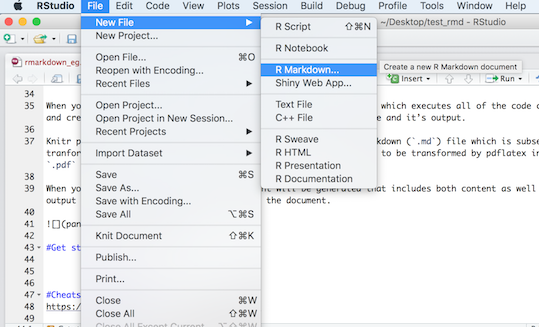
\includegraphics[width=5.20833in]{../figures/getstarted.png}\\
\hspace*{0.333em}\\
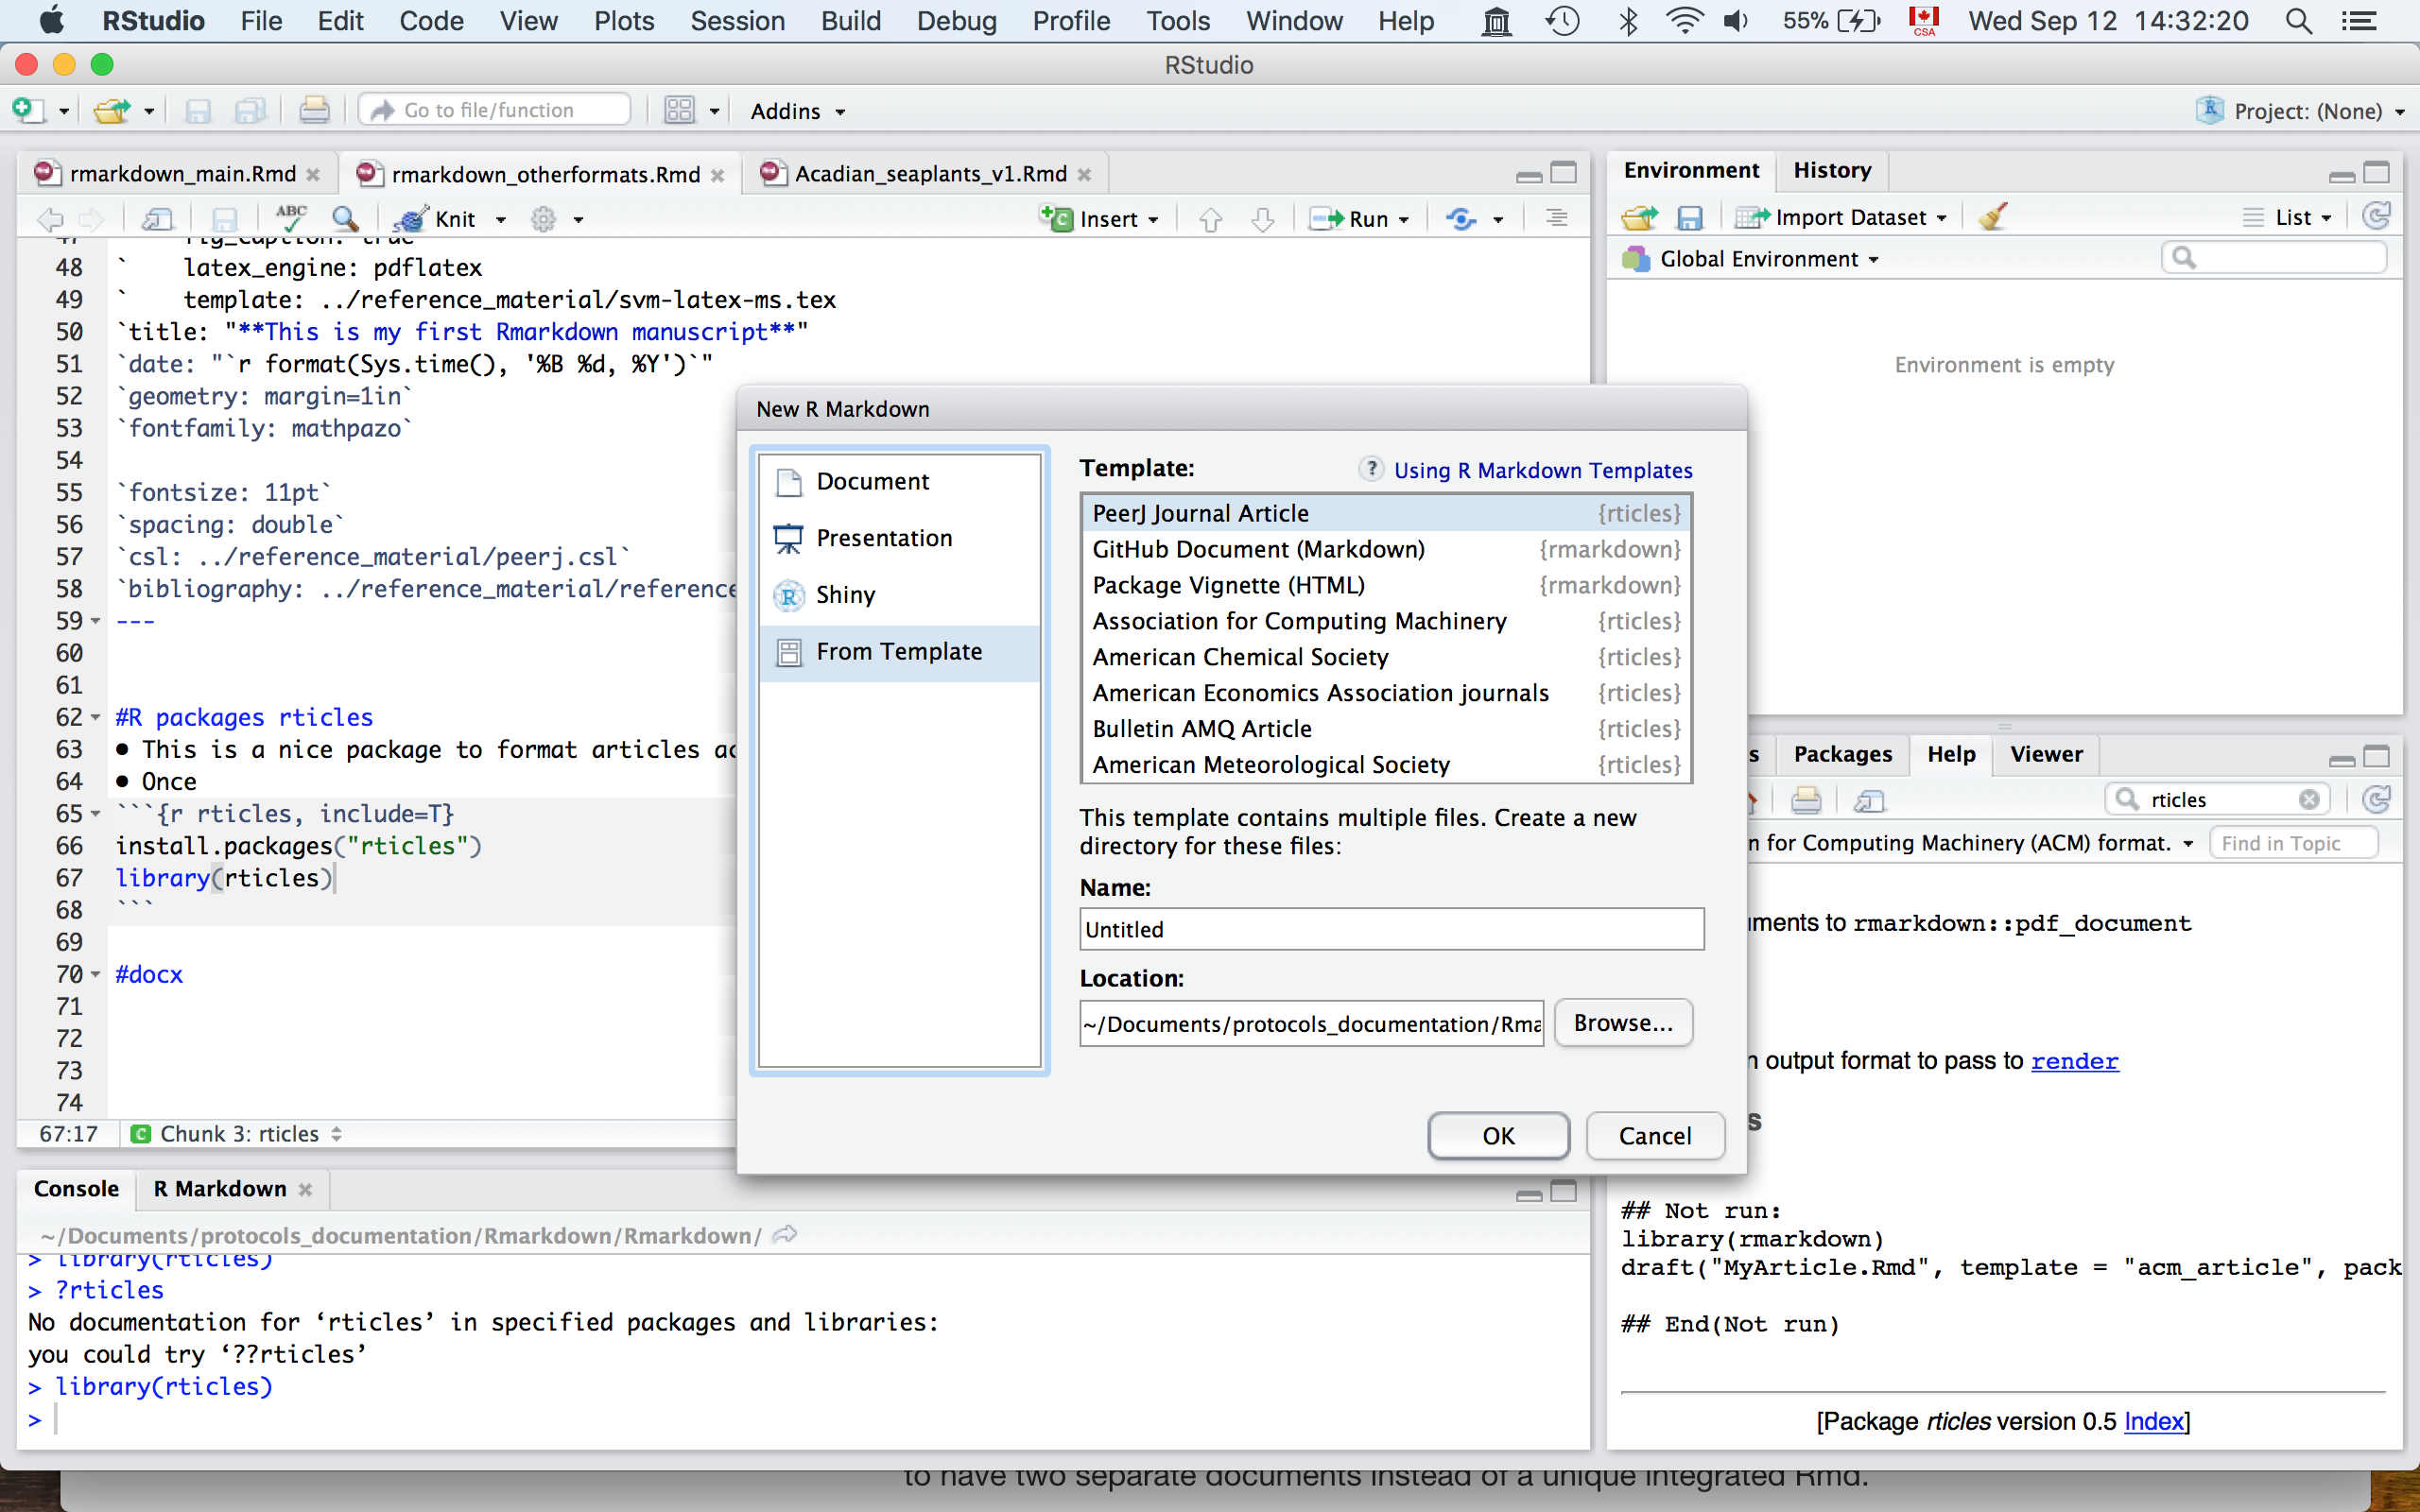
\includegraphics[width=5.20833in]{../figures/from_template.png}\\
\hspace*{0.333em}

\section{\texorpdfstring{Template
(\emph{.tex})}{Template (.tex)}}\label{template-.tex}

\begin{itemize}
\item
  You can build your own template if you know Latex\ldots{}
\item
  There are many templates available on the web that you can use.
\item
  Here is one I like for
  \href{https://github.com/svmiller/svm-r-markdown-templates/blob/master/svm-latex-ms.tex}{manuscripts}
  (Thanks svmiller!):
\item
  Here is one I like for
  \href{https://github.com/svmiller/svm-r-markdown-templates/blob/master/svm-latex-cv.tex}{CVs}:
\item
  Simply download it and add it to the YAML header like this:
  \texttt{template:\ ../reference\_material/svm-latex-ms.tex}\\
  \texttt{-\/-\/-}\\
  \texttt{output:}\\
  \texttt{pdf\_document:}\\
  \texttt{keep\_tex:\ true}\\
  \texttt{fig\_caption:\ true}\\
  \texttt{latex\_engine:\ pdflatex}\\
  \texttt{template:\ ../reference\_material/svm-latex-ms.tex}\\
  \texttt{title:\ "**This\ is\ my\ first\ Rmarkdown\ manuscript**}\\
  \texttt{-\/-\/-}
\end{itemize}

\section{Overleaf}\label{overleaf}

\begin{itemize}
\tightlist
\item
  Overleaf is an online LaTeX and Rich Text collaborative writing and
  publishing tool that makes the whole process of writing, editing and
  publishing scientific documents much quicker and easier.
\end{itemize}

\begin{figure}
\centering
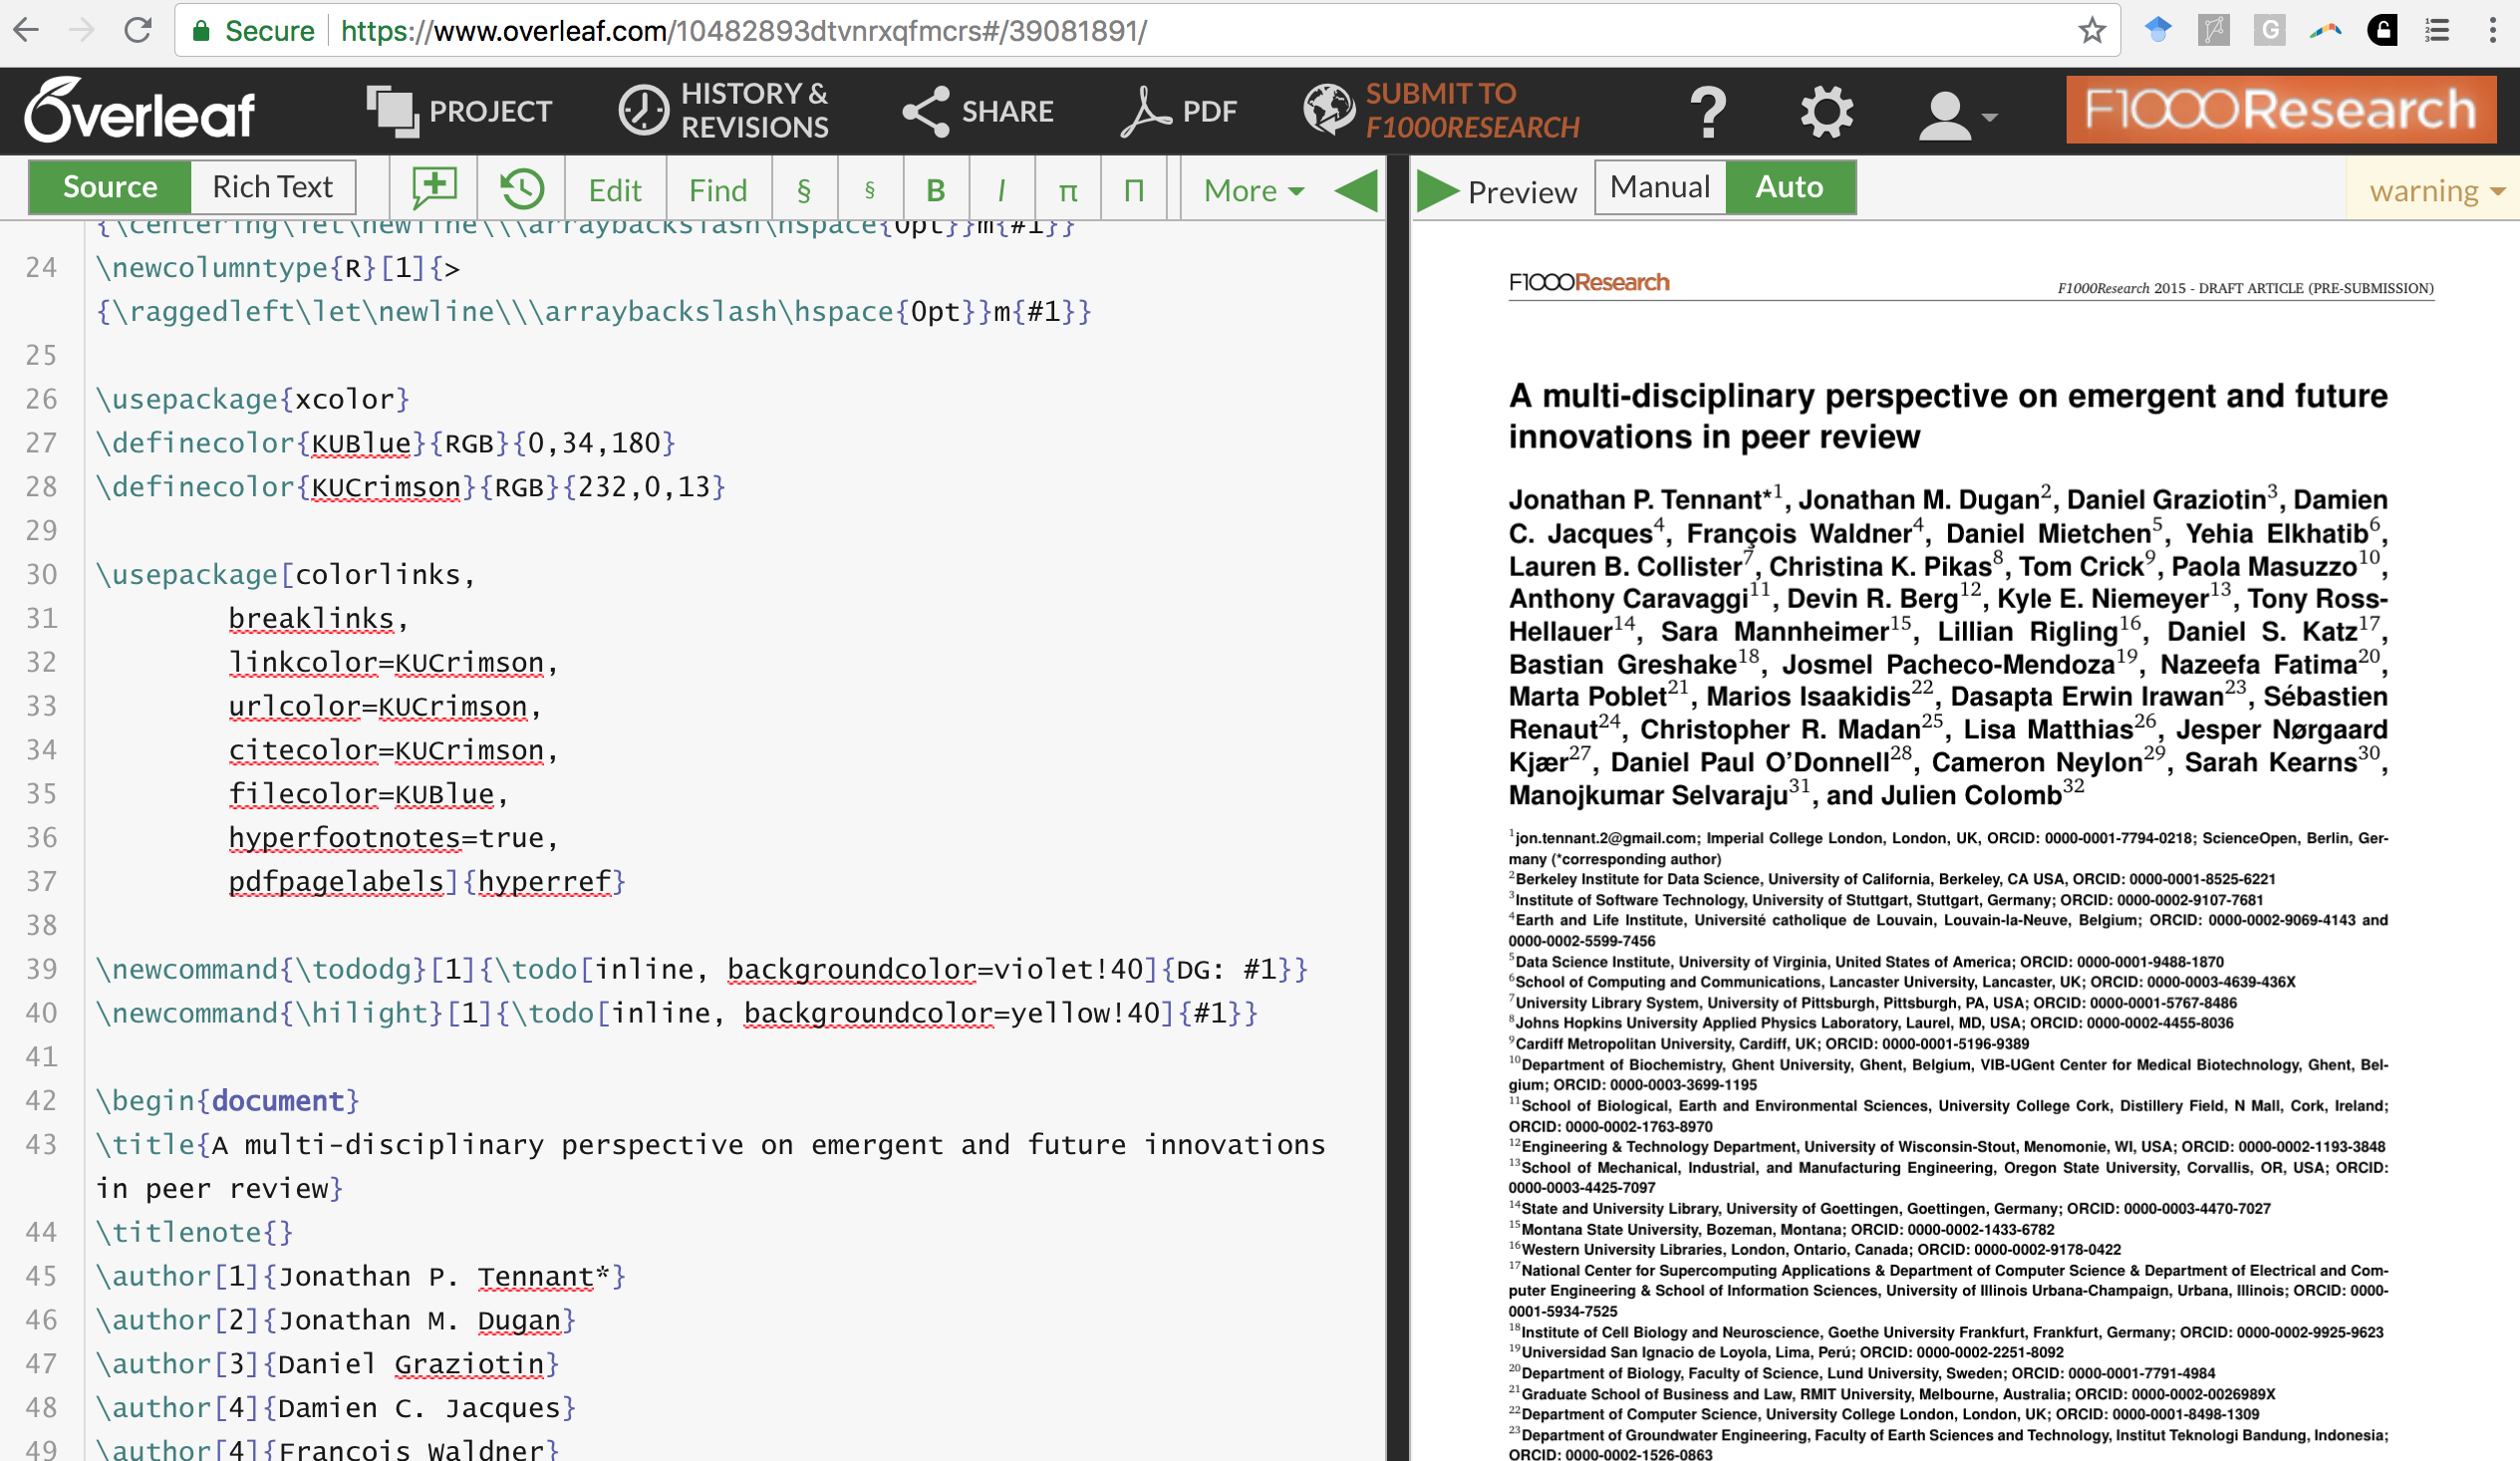
\includegraphics[width=5.20833in]{../figures/overleaf.png}
\caption{}
\end{figure}

\begin{itemize}
\item
  Remember this:\\
  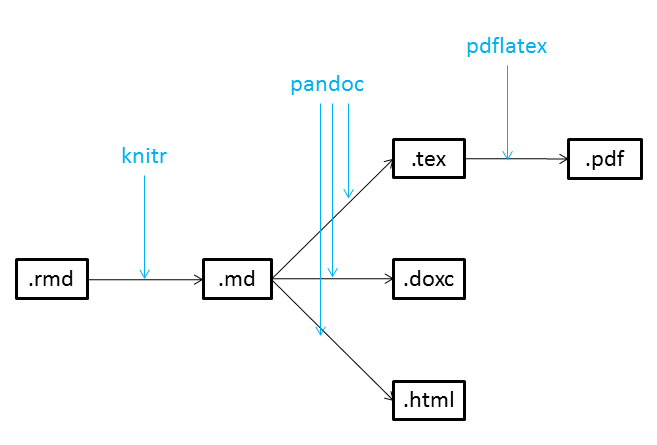
\includegraphics[width=5.20833in]{../figures/pandoc1.png}
\item
  So you can generate your \textbf{.tex} file, upload it to a github
  repo and Overleaf will connect to it. Others can then collaborate and
  modify the .tex file.
\item
  Let's quickly look at \href{https://www.overleaf.com/}{overleaf}.
\item
  \href{https://medium.com/@arinbasu/a-tutorial-on-how-to-interface-an-r-notebook-with-overleaf-11f23c306cfd}{A
  tutorial on how to interface an R Notebook with Overleaf}
\item
  {[}How do I connect an Overleaf project with a repo on GitHub, GitLab
  or BitBucket?{]}
  \url{https://www.overleaf.com/learn/how-to/How_do_I_connect_an_Overleaf_project_with_a_repo_on_GitHub,_GitLab_or_BitBucket\%3F}
\end{itemize}

\section{slide presentation}\label{slide-presentation}

\begin{itemize}
\tightlist
\item
  You can generate Powerpoint like presentations. We will not learn this
  today: 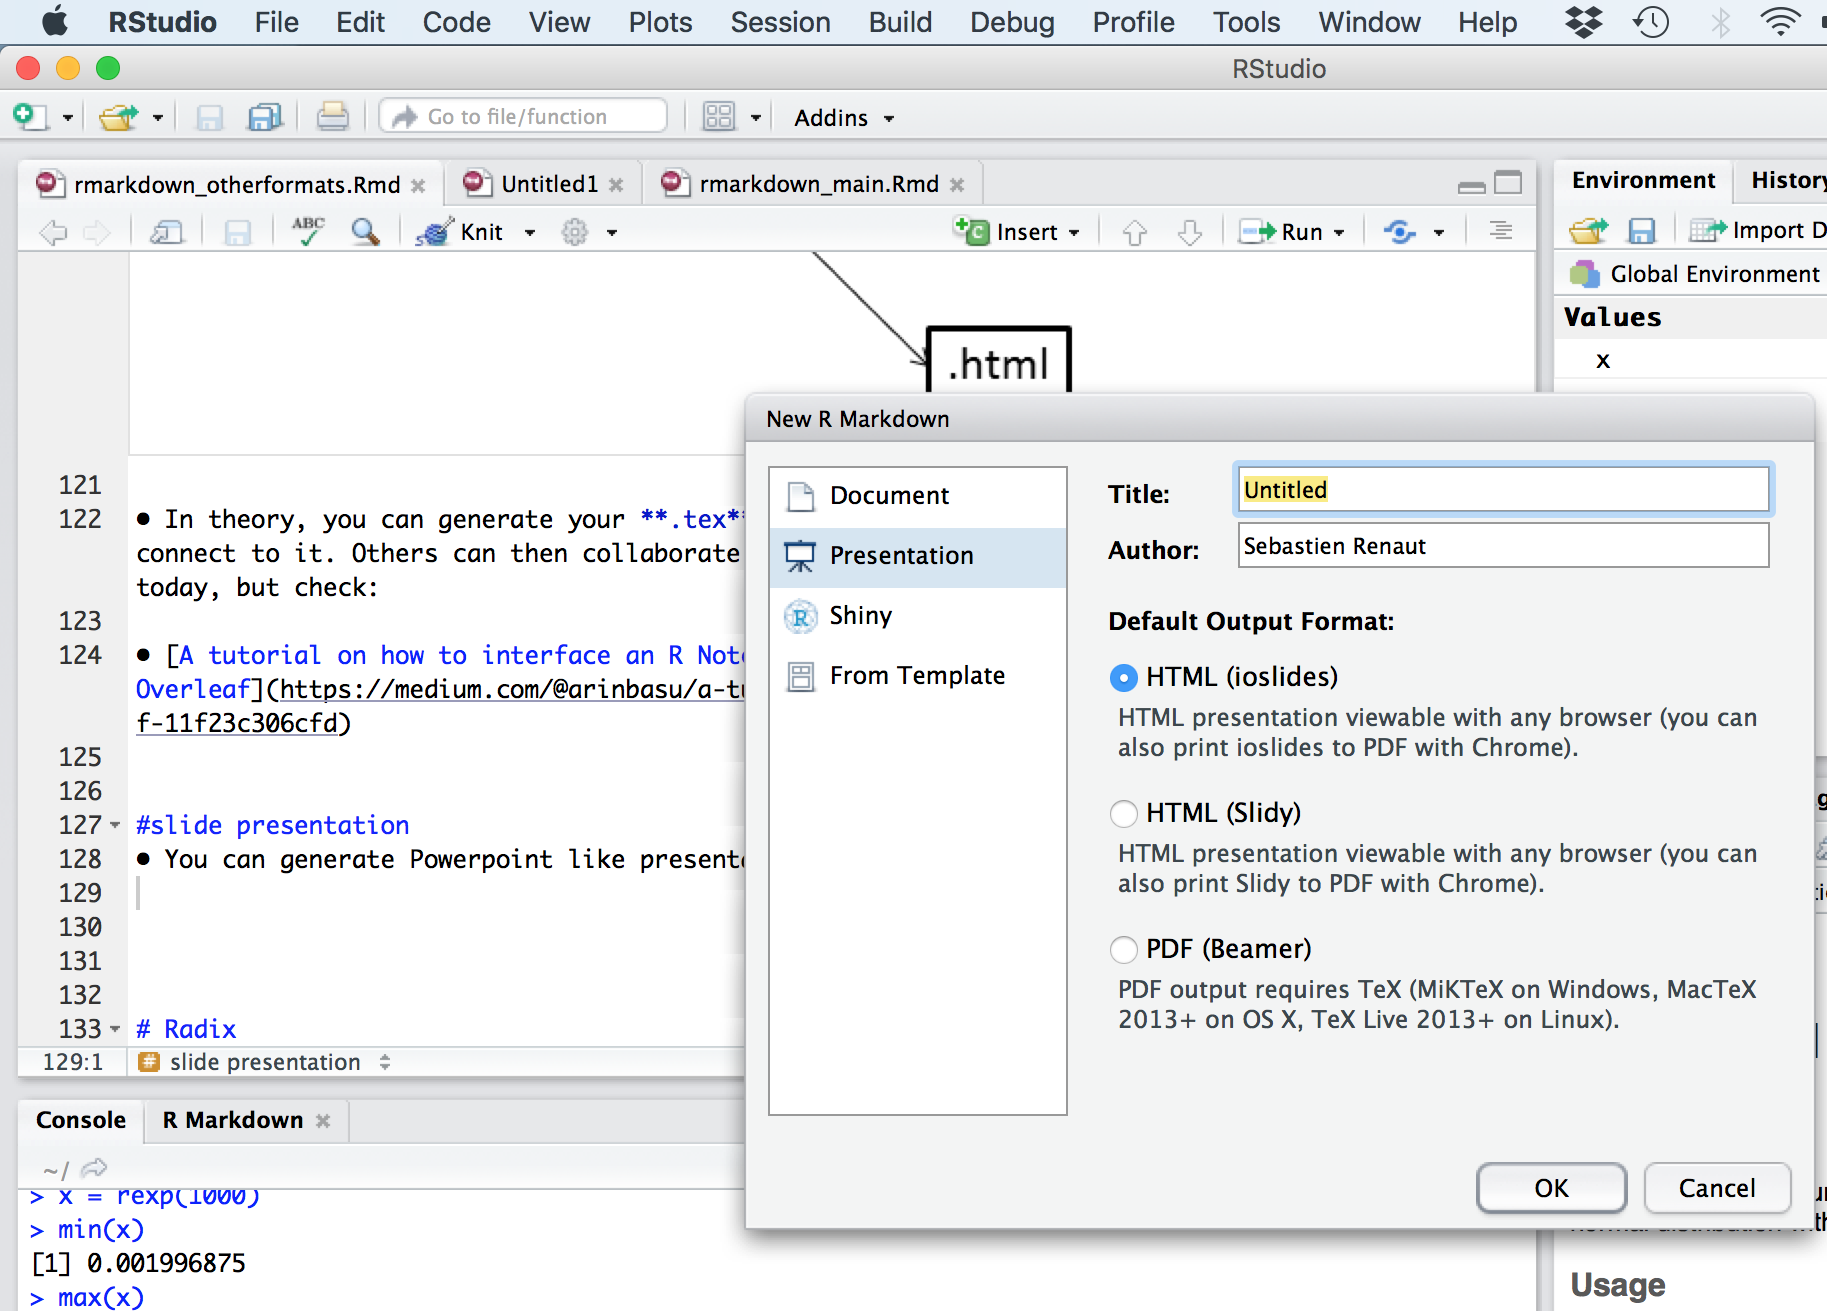
\includegraphics[width=5.20833in]{../figures/slides.png}
\end{itemize}

\section{Bookdown}\label{bookdown}

\url{https://bookdown.org/}

\section{Radix}\label{radix}

\begin{itemize}
\item
  \url{https://blog.rstudio.com/2018/09/19/radix-for-r-markdown/}
\item
  Stay tuned, as it might replace the `rmarkdown' package\ldots{}\\
  
\includegraphics[width=5.20833in]{../figures/radix.png}
\end{itemize}


\end{document}
